\subsection{Triggers}

This section presents the triggers implemented in the Steam Store Management database. According to the assignment requirement, two categories of triggers must be provided: one trigger that enforces a \textbf{business constraint} which cannot be expressed directly inside table creation statements, and one or more triggers that compute the value of a \textbf{derived attribute}.

The first part introduces the constraint trigger \texttt{trg\_review\_only\_owned\_game}, which enforces the semantic rule that a player may submit a review for a game only if that game already exists in the player's library. The second part introduces a chain of triggers that maintain two derived attributes: \texttt{effective\_price} in the \texttt{GAME} table and \texttt{price\_at\_purchase} in the \texttt{CONTAINS} table.

\subsubsection{Business Constraint Trigger}

A semantic constraint identified in Section~1.3 states that \emph{a player may write a review for a game only if that game already exists in the player's account or library}. This rule cannot be enforced directly with a CHECK constraint inside the \texttt{REVIEW} table, because verifying it requires looking up rows in another table (\texttt{OWNS\_LIBRARY}) at the moment a review is inserted or updated. Therefore, a trigger is the appropriate mechanism to enforce this business rule.

\paragraph{DML operations that may violate the constraint.}
The constraint can be violated by two DML operations on the \texttt{REVIEW} table: an \texttt{INSERT} that adds a new review for a game the player does not own, and an \texttt{UPDATE} that changes the \texttt{game\_id} or \texttt{user\_id} of an existing review so that the new combination is no longer present in \texttt{OWNS\_LIBRARY}. Two triggers are therefore implemented, one for each operation.

\paragraph{Trigger implementation.}
The trigger queries the \texttt{OWNS\_LIBRARY} table to check whether a row with the same \texttt{user\_id} and \texttt{game\_id} as the new review exists. If no such row is found, the trigger raises a \texttt{SIGNAL SQLSTATE '45000'} with a meaningful error message instead of allowing the invalid review to be inserted or updated.

\begin{lstlisting}[language=SQL, caption={Trigger enforcing the business rule that reviews are allowed only for owned games}, label={lst:trg-review-owned}]
DELIMITER //

CREATE TRIGGER trg_review_only_owned_game_insert
BEFORE INSERT ON REVIEW
FOR EACH ROW
BEGIN
    DECLARE v_owned INT DEFAULT 0;

    SELECT COUNT(*) INTO v_owned
    FROM OWNS_LIBRARY
    WHERE player_id = NEW.player_id
      AND game_id   = NEW.game_id;

    IF v_owned = 0 THEN
        SIGNAL SQLSTATE '45000'
        SET MESSAGE_TEXT =
          'Constraint Violation: A player may only review a game they own in their library.';
    END IF;
END //

CREATE TRIGGER trg_review_only_owned_game_update
BEFORE UPDATE ON REVIEW
FOR EACH ROW
BEGIN
    DECLARE v_owned INT DEFAULT 0;

    IF NEW.player_id <> OLD.player_id OR NEW.game_id <> OLD.game_id THEN
        SELECT COUNT(*) INTO v_owned
        FROM OWNS_LIBRARY
        WHERE player_id = NEW.player_id
          AND game_id   = NEW.game_id;

        IF v_owned = 0 THEN
            SIGNAL SQLSTATE '45000'
            SET MESSAGE_TEXT =
              'Constraint Violation: Updated review must still refer to a game owned by the player.';
        END IF;
    END IF;
END //

DELIMITER ;
\end{lstlisting}

\paragraph{Test cases for the constraint trigger.}

\begin{table}[H]
\centering
\caption{Test cases for the review-only-on-owned-game constraint trigger}
\label{tab:trg-review-owned-tests}
\begin{tabular}{|c|p{6.5cm}|p{5cm}|}
\hline
\textbf{No.} & \textbf{Test scenario} & \textbf{Expected outcome} \\ \hline
1 & A player attempts to review a game that exists in their \texttt{OWNS\_LIBRARY}. & Review is inserted successfully. \\ \hline
2 & A player attempts to review a game that does \emph{not} exist in their \texttt{OWNS\_LIBRARY}. & Trigger raises error \texttt{45000} with the message ``A player may only review a game they own in their library.'' \\ \hline
3 & An existing review is updated to point to a different game that the player does \emph{not} own. & Update is rejected by \texttt{trg\_review\_only\_owned\_game\_update}. \\ \hline
\end{tabular}
\end{table}

\begin{lstlisting}[language=SQL, caption={Sample SQL statements to demonstrate the constraint trigger}, label={lst:trg-review-owned-demo}]
USE SteamDB;

-- =========================================================
-- Test 1 (VALID): player_id = 1 owns game_id = 2 in OWNS_LIBRARY,
-- and no review exists yet for (1, 2). The trigger allows the insert.
-- =========================================================
INSERT INTO `REVIEW` (rating, comment, review_date, player_id, game_id)
VALUES ('Recommended', 'Trigger Test - valid case', CURDATE(), 1, 2);

SELECT review_id, player_id, game_id, rating, comment
FROM `REVIEW`
WHERE player_id = 1 AND game_id = 2;
-- Expected: 1 row inserted successfully.


-- =========================================================
-- Test 2 (INVALID INSERT): player_id = 1 does NOT own game_id = 7
-- (player 1 only owns games 2 and 3 in OWNS_LIBRARY).
-- The trigger must reject the insert.
-- =========================================================
INSERT INTO `REVIEW` (rating, comment, review_date, player_id, game_id)
VALUES ('Recommended', 'Trigger Test - should fail', CURDATE(), 1, 7);
-- Expected:
-- ERROR 1644 (45000): Constraint Violation: A player may only review
-- a game they own in their library.


-- =========================================================
-- Test 3 (INVALID UPDATE): change the review just inserted in Test 1
-- (player 1, game 2) so that it now points to game 7 - which player 1
-- does NOT own. The UPDATE trigger must reject the change.
-- =========================================================
UPDATE `REVIEW`
SET game_id = 7
WHERE player_id = 1 AND game_id = 2;
-- Expected:
-- ERROR 1644 (45000): Constraint Violation: Updated review must still refer
-- to a game owned by the player.


-- =========================================================
-- Cleanup (optional): remove the test review inserted in Test 1
-- so the database returns to its original state.
-- =========================================================
DELETE FROM `REVIEW`
WHERE player_id = 1 AND game_id = 2 AND comment = 'Trigger Test - valid case';
\end{lstlisting}

\paragraph{Execution result.}
The screenshots below show the execution of the three test cases inside the MySQL client. Test~1 (Figure~\ref{fig:trg-review-owned-result1}) inserts a new review for player~1 and game~2 successfully because player~1 owns game~2 in \texttt{OWNS\_LIBRARY}; the subsequent \texttt{SELECT} confirms that the row was created with \texttt{review\_id = 11}. Test~2 (Figure~\ref{fig:trg-review-owned-result2}) attempts to insert a review for player~1 on game~7, which is not owned by player~1; the trigger rejects the operation with \texttt{SQL Error 1644 [45000]: Constraint Violation: A player may only review a game they own in their library}. Test~3 (Figure~\ref{fig:trg-review-owned-result3}) attempts to update the review just inserted in Test~1 so that its \texttt{game\_id} becomes 7; the update trigger rejects the change with \texttt{SQL Error 1644 [45000]: Constraint Violation: Updated review must still refer to a game owned by the player}.

\begin{figure}[H]
    \centering
    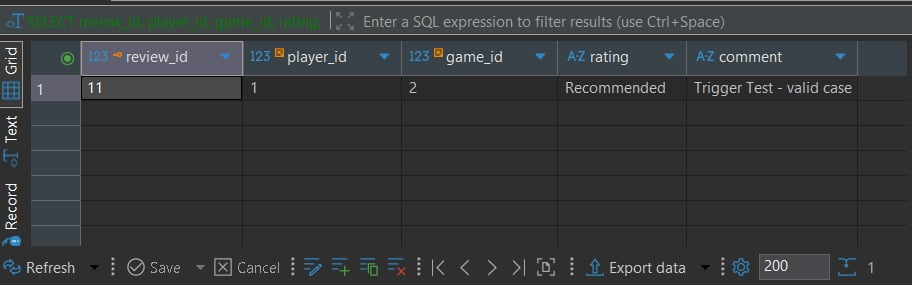
\includegraphics[width=0.9\linewidth]{graphics/trigger_review_owned_result1.jpg}
    \caption{Test~1 result --- valid insert succeeds (player~1 owns game~2)}
    \label{fig:trg-review-owned-result1}
\end{figure}

\begin{figure}[H]
    \centering
    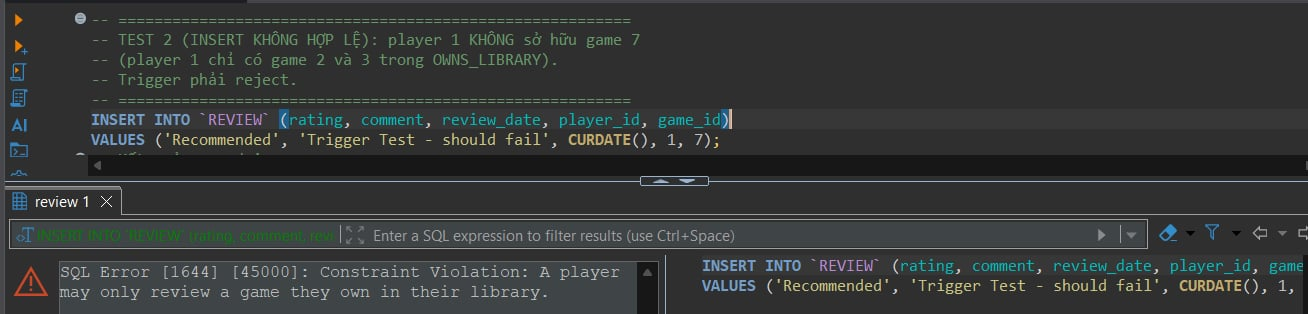
\includegraphics[width=0.9\linewidth]{graphics/trigger_review_owned_result2.jpg}
    \caption{Test~2 result --- invalid insert rejected by \texttt{trg\_review\_only\_owned\_game\_insert}}
    \label{fig:trg-review-owned-result2}
\end{figure}

\begin{figure}[H]
    \centering
    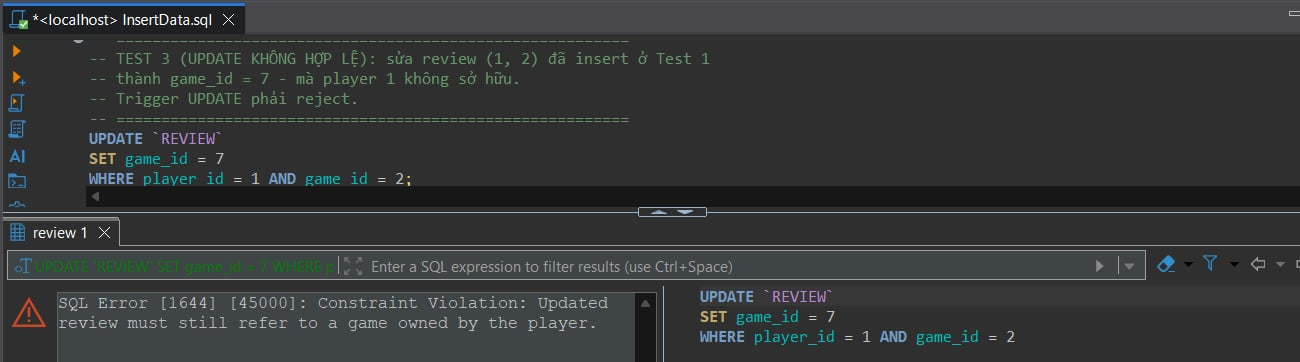
\includegraphics[width=0.9\linewidth]{graphics/trigger_review_owned_result3.jpg}
    \caption{Test~3 result --- invalid update rejected by \texttt{trg\_review\_only\_owned\_game\_update}}
    \label{fig:trg-review-owned-result3}
\end{figure}

\subsubsection{Chosen Derived Attribute}

The chosen derived attribute is \texttt{price\_at\_purchase} from the \texttt{CONTAINS} relationship table. 
This attribute stores the price of a game at the moment of purchase. 
It is important because the price of a game may change later due to base price updates or promotions, but historical transaction records must preserve the exact price paid at the time of purchase.

The value of \texttt{price\_at\_purchase} is derived from the current \texttt{effective\_price} of the corresponding game. 
If \texttt{effective\_price} is not available, the system falls back to the game's \texttt{base\_price}.
\subsubsection{DML Operations Affecting the Derived Attributes}

Since \texttt{price\_at\_purchase} depends on \texttt{effective\_price}, the triggers must handle both attributes. 
Table~\ref{tab:dml-effective-price} shows the DML operations that affect \texttt{effective\_price}.

\begin{table}[H]
\centering
\caption{DML operations affecting \texttt{effective\_price}}
\label{tab:dml-effective-price}
\begin{tabular}{|l|l|p{8cm}|}
\hline
\textbf{DML Operation} & \textbf{Table} & \textbf{Reason} \\ \hline
Insert & \texttt{GAME} & A newly inserted game has no promotion, so its \texttt{effective\_price} is initialized using its \texttt{base\_price}. \\ \hline
Update & \texttt{GAME} & When \texttt{base\_price} changes, the \texttt{effective\_price} must be recalculated. \\ \hline
Insert & \texttt{GAME\_PROMOTION} & When a promotion is assigned to a game, the \texttt{effective\_price} may change. \\ \hline
Delete & \texttt{PROMOTION} & When a promotion is removed, affected games must recalculate their \texttt{effective\_price}. \\ \hline
\end{tabular}
\end{table}

Table~\ref{tab:dml-price-at-purchase} shows the DML operation that affects \texttt{price\_at\_purchase}.

\begin{table}[H]
\centering
\caption{DML operation affecting \texttt{price\_at\_purchase}}
\label{tab:dml-price-at-purchase}
\begin{tabular}{|l|l|p{8cm}|}
\hline
\textbf{DML Operation} & \textbf{Table} & \textbf{Reason} \\ \hline
Insert & \texttt{CONTAINS} & When a game is inserted into a transaction, the current \texttt{effective\_price} must be copied into \texttt{price\_at\_purchase}. \\ \hline
\end{tabular}
\end{table}
\subsubsection{Full SQL Implementation}

The following SQL script shows the triggers used to maintain \texttt{effective\_price} and \texttt{price\_at\_purchase}.

\begin{lstlisting}[language=SQL, caption={Triggers for maintaining effective price and price at purchase}, label={lst:price-triggers}]
DELIMITER //

CREATE TRIGGER trg_contains_set_price
BEFORE INSERT ON CONTAINS
FOR EACH ROW
BEGIN
    DECLARE v_effective_price DECIMAL(10,2);

    SELECT COALESCE(effective_price, base_price) INTO v_effective_price
    FROM GAME 
    WHERE game_id = NEW.game_id;

    SET NEW.price_at_purchase = v_effective_price;
END //

DELIMITER ;

DELIMITER //

CREATE TRIGGER trg_game_insert_price
BEFORE INSERT ON GAME
FOR EACH ROW
BEGIN
    SET NEW.effective_price = NEW.base_price;
END //

DELIMITER ;

DELIMITER //

CREATE TRIGGER trg_update_game_price
BEFORE UPDATE ON GAME
FOR EACH ROW
BEGIN
    DECLARE v_discount DECIMAL(5,2);

    IF OLD.base_price <> NEW.base_price THEN
        SELECT COALESCE(MAX(p.discount_percentage), 0)
        INTO v_discount
        FROM PROMOTION p
        JOIN GAME_PROMOTION gp ON p.promotion_id = gp.promotion_id
        WHERE gp.game_id = NEW.game_id 
          AND CURDATE() BETWEEN p.start_date AND p.end_date;

        SET NEW.effective_price = ROUND(NEW.base_price * (1 - v_discount / 100), 2);
    END IF;
END //

DELIMITER ;

DELIMITER //

CREATE TRIGGER trg_gamepromotion_insert
AFTER INSERT ON GAME_PROMOTION
FOR EACH ROW
BEGIN
    DECLARE v_discount DECIMAL(5,2);

    SELECT COALESCE(MAX(p.discount_percentage), 0)
    INTO v_discount
    FROM PROMOTION p
    JOIN GAME_PROMOTION gp 
        ON p.promotion_id = gp.promotion_id
    WHERE gp.game_id = NEW.game_id 
      AND CURDATE() BETWEEN p.start_date AND p.end_date;

    UPDATE GAME
    SET effective_price = ROUND(base_price * (1 - v_discount / 100), 2)
    WHERE game_id = NEW.game_id;
END //

DELIMITER ;

DELIMITER //

CREATE TRIGGER trg_promotion_delete
BEFORE DELETE ON PROMOTION
FOR EACH ROW
BEGIN
    DECLARE done INT DEFAULT 0;
    DECLARE v_game_id INT;
    DECLARE v_base_price DECIMAL(10,2);
    DECLARE v_discount DECIMAL(5,2);

    DECLARE game_cursor CURSOR FOR
        SELECT g.game_id, g.base_price
        FROM GAME g
        JOIN GAME_PROMOTION gp ON g.game_id = gp.game_id
        WHERE gp.promotion_id = OLD.promotion_id;

    DECLARE CONTINUE HANDLER FOR NOT FOUND SET done = 1;

    OPEN game_cursor;

    read_loop: LOOP
        FETCH game_cursor INTO v_game_id, v_base_price;
        IF done THEN 
            LEAVE read_loop; 
        END IF;

        SELECT COALESCE(MAX(p.discount_percentage), 0) 
        INTO v_discount
        FROM PROMOTION p
        JOIN GAME_PROMOTION gp2 ON p.promotion_id = gp2.promotion_id
        WHERE gp2.game_id = v_game_id
          AND p.promotion_id <> OLD.promotion_id
          AND CURDATE() BETWEEN p.start_date AND p.end_date;

        UPDATE GAME
        SET effective_price = ROUND(v_base_price * (1 - v_discount / 100), 2)
        WHERE game_id = v_game_id;

    END LOOP;

    CLOSE game_cursor;
END //

DELIMITER ;
\end{lstlisting}
\subsubsection{Trigger Explanation}

The trigger \texttt{trg\_game\_insert\_price} is executed before a new game is inserted into the \texttt{GAME} table. 
Since a newly inserted game has no promotion applied yet, its \texttt{effective\_price} is initialized with the same value as its \texttt{base\_price}.

The trigger \texttt{trg\_update\_game\_price} is executed before a row in the \texttt{GAME} table is updated. 
When the \texttt{base\_price} changes, the trigger retrieves the highest active discount percentage among all valid promotions associated with that game. 
The \texttt{effective\_price} is then recalculated using the updated base price and the best available discount.

The trigger \texttt{trg\_gamepromotion\_insert} is executed after a new record is inserted into the \texttt{GAME\_PROMOTION} table. 
When a promotion is assigned to a game, this trigger updates the game’s \texttt{effective\_price}. 
If multiple active promotions are available, the highest discount percentage is selected using the \texttt{MAX} function.

The trigger \texttt{trg\_promotion\_delete} is executed before a promotion is deleted from the \texttt{PROMOTION} table. 
Since one promotion may affect multiple games, a cursor is used to iterate through all affected games. 
For each game, the trigger recalculates the \texttt{effective\_price} using the highest remaining active promotion. 
If no valid promotion remains, the discount defaults to 0.

Finally, the trigger \texttt{trg\_contains\_set\_price} is executed before a new record is inserted into the \texttt{CONTAINS} table. 
It copies the current \texttt{effective\_price} of the game into \texttt{price\_at\_purchase}. 
This ensures that each transaction stores the exact game price at the moment of purchase and preserves historical accuracy even if the game price changes later.
\subsubsection{Test Cases}

The following SQL statements were used to test the trigger behavior.

\begin{lstlisting}[language=SQL, caption={Test cases for price-related triggers}, label={lst:price-trigger-test}]
USE steam_store;

-- Test 1: Check that effective_price is initialized
-- when a new game is inserted
INSERT INTO `GAME` (
    title, base_price, release_date, graphics, os, processor, memory, developer_id
)
VALUES (
    'Trigger Test Game',
    1000000.00,
    '2026-06-01',
    'GTX 1050',
    'Windows 10',
    'Intel i5',
    '8GB RAM',
    6
);

SET @test_game_id = LAST_INSERT_ID();

SELECT 
    game_id, 
    title, 
    base_price, 
    effective_price
FROM `GAME`
WHERE game_id = @test_game_id;

-- Test 2: Apply an active promotion to the game
INSERT INTO `PROMOTION` (
    name, discount_percentage, start_date, end_date
)
VALUES (
    'Trigger Test Promotion',
    20.00,
    CURDATE(),
    DATE_ADD(CURDATE(), INTERVAL 10 DAY)
);

SET @test_promotion_id = LAST_INSERT_ID();

INSERT INTO `GAME_PROMOTION` (game_id, promotion_id)
VALUES (@test_game_id, @test_promotion_id);

SELECT 
    game_id, 
    title, 
    base_price, 
    effective_price
FROM `GAME`
WHERE game_id = @test_game_id;

-- Test 3: Insert the game into a transaction
INSERT INTO `TRANSACTION` (
    date, payment_method, total_amount, player_id
)
VALUES (
    NOW(),
    'Credit Card',
    800000.00,
    1
);

SET @test_transaction_id = LAST_INSERT_ID();

INSERT INTO `CONTAINS` (
    transaction_id, game_id, price_at_purchase
)
VALUES (
    @test_transaction_id,
    @test_game_id,
    0
);

SELECT 
    transaction_id, 
    game_id, 
    price_at_purchase
FROM `CONTAINS`
WHERE transaction_id = @test_transaction_id
  AND game_id = @test_game_id;
\end{lstlisting}
\subsubsection{Execution Result}

The test results show that the triggers correctly maintain both derived attributes. 
First, when a new game is inserted into the \texttt{GAME} table, its \texttt{effective\_price} is initialized from the \texttt{base\_price}. 
Then, when an active promotion with a 20\% discount is assigned to the game, the \texttt{effective\_price} is automatically recalculated from 1,000,000.00 to 800,000.00. 
Finally, when the game is inserted into a transaction through the \texttt{CONTAINS} table, the current \texttt{effective\_price} is copied into \texttt{price\_at\_purchase}.

\begin{figure}[H]
    \centering
    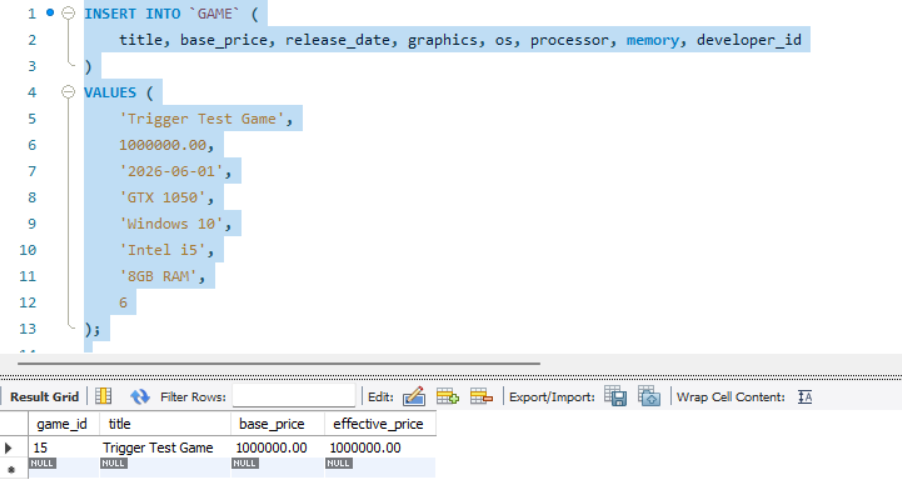
\includegraphics[width=0.9\linewidth]{graphics/trigger_effective_price_result.png}
    \caption{Trigger result after applying an active promotion to update \texttt{effective\_price}}
    \label{fig:trigger-effective-price-result}
\end{figure}

\begin{figure}[H]
    \centering
    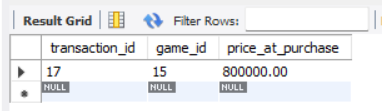
\includegraphics[width=0.65\linewidth]{graphics/trigger-price-at-purchase-result.png}
    \caption{Trigger result for storing \texttt{price\_at\_purchase} in the \texttt{CONTAINS} table}
    \label{fig:trigger-price-at-purchase-result}
\end{figure}